\documentclass[11pt,a4paper]{article}

\usepackage[headsep=1cm,headheight=3cm,left=3.5cm,right=3.5cm,top=2.5cm,bottom=2.5cm,a4paper]{geometry}

\linespread{1.3}
\setlength{\parindent}{0pt}
\setlength{\parskip}{1em}

\usepackage[spanish]{babel}
\usepackage[utf8]{inputenc}

%% Fuentes personalizadas para utilizar con XeTeX
\usepackage[sfdefault]{roboto}
\usepackage[scaled=0.9]{DejaVuSansMono}
\usepackage[T1]{fontenc}

\usepackage{enumitem}
\setlist[itemize]{leftmargin=*}
\setlist[enumerate]{leftmargin=*}

\usepackage{changepage}

\newcommand{\term}[2]{\textbf{#1}\quad#2}

\newcounter{ActCounter}
\newcommand{\act}[1]{\addtocounter{ActCounter}{1}\textbf{\sffamily ACT-\theActCounter}\quad#1\\}

\newcounter{CUCounter}
\newcommand{\cu}[1]{\addtocounter{CUCounter}{1}\textbf{\sffamily CU-\theCUCounter}\quad#1\\}

\usepackage{tabularx}
\usepackage{float}
\usepackage{adjustbox}

\title{Práctica 3: Análisis y especificación de requisitos \large\\ Fundamentos de Ingeniería del Software}
\author{Sofía Almedia Bruno \and José Antonio Álvarez Ocete \and Miguel Lentisco Ballesteros \and Simón López Vico \and José María Martín Luque}

\begin{document}

\maketitle

\section{Diagrama de clases}

\begin{figure}[H]
	\caption{Diagrama de clases}
	\centering
  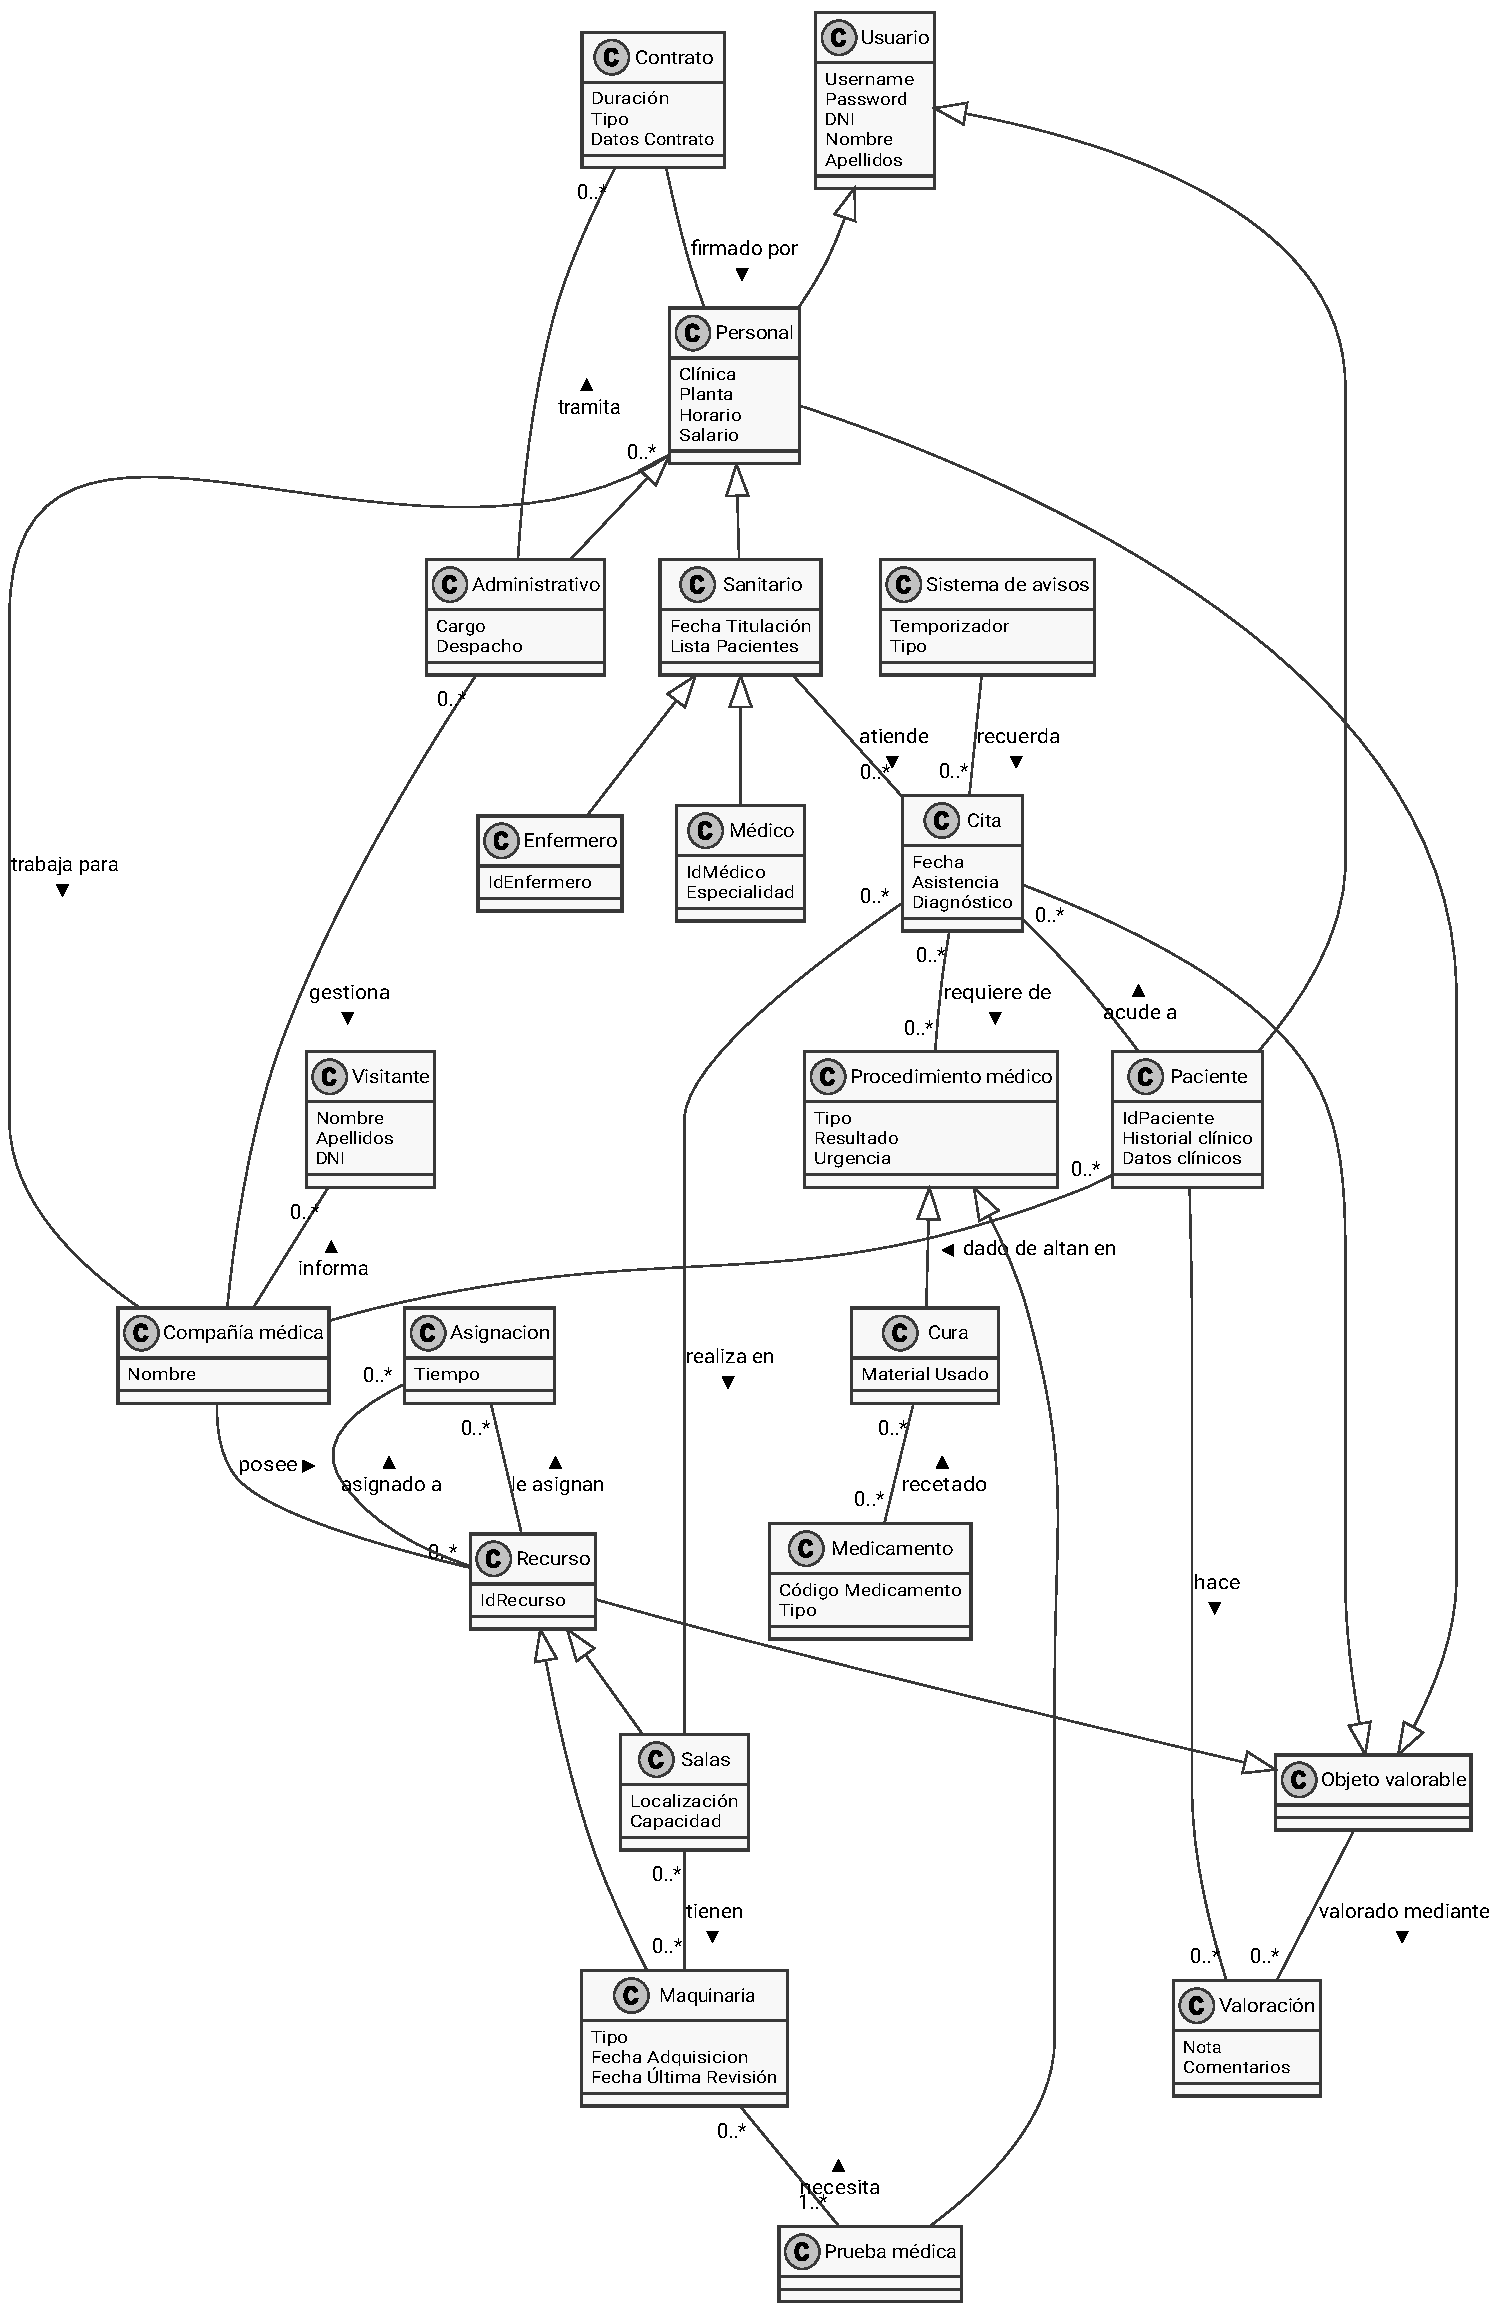
\includegraphics[width=\textwidth,height=\textheight,keepaspectratio]{diagramas/pdf/diagramaClases.pdf}
\end{figure}

\section{Diagramas de secuencia}

\begin{figure}[H]
	\caption{Consulta}
	\centering
  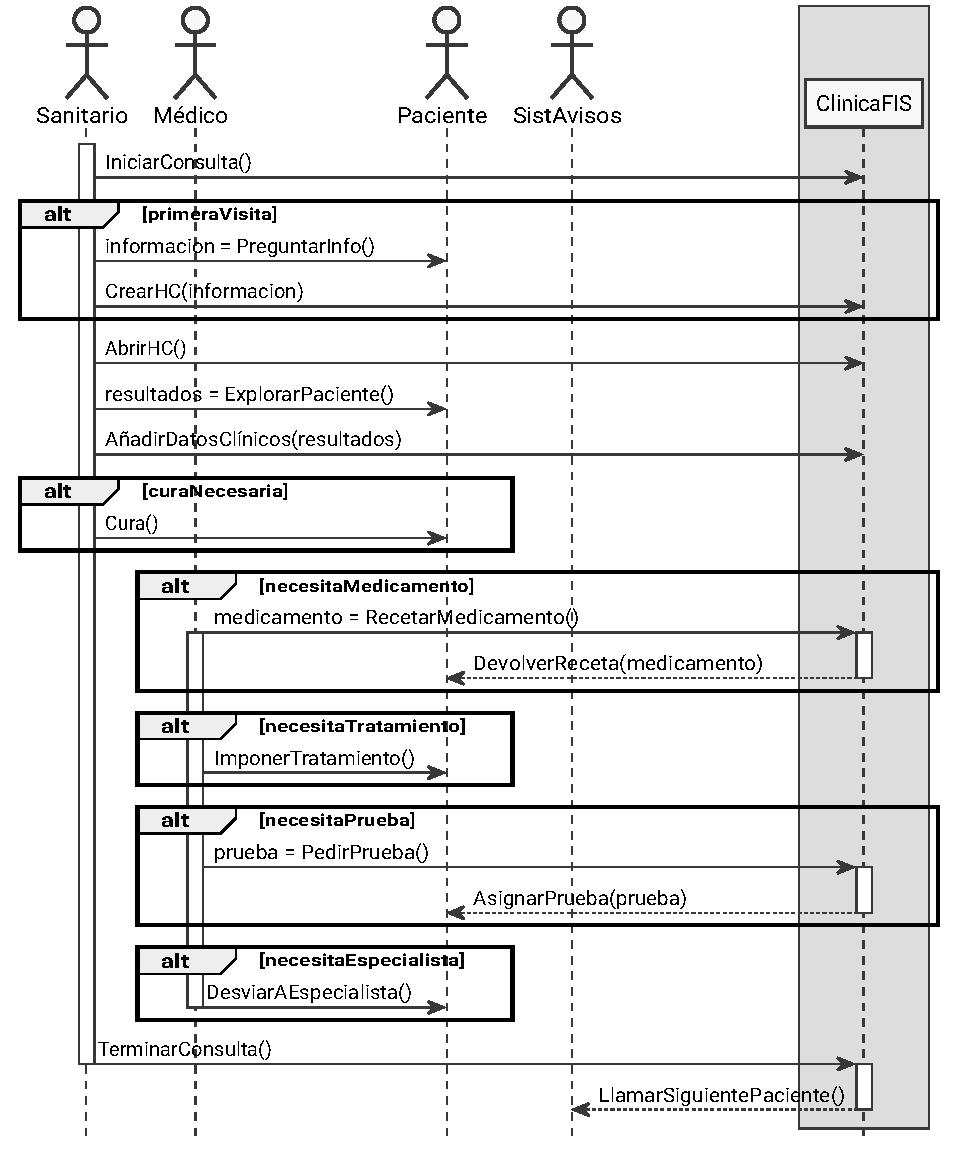
\includegraphics[width=\textwidth,height=\textheight,keepaspectratio]{diagramas/pdf/diagramaConsulta.pdf}
\end{figure}

\begin{figure}[H]
	\caption{Gestión de Consulta}
	\centering
	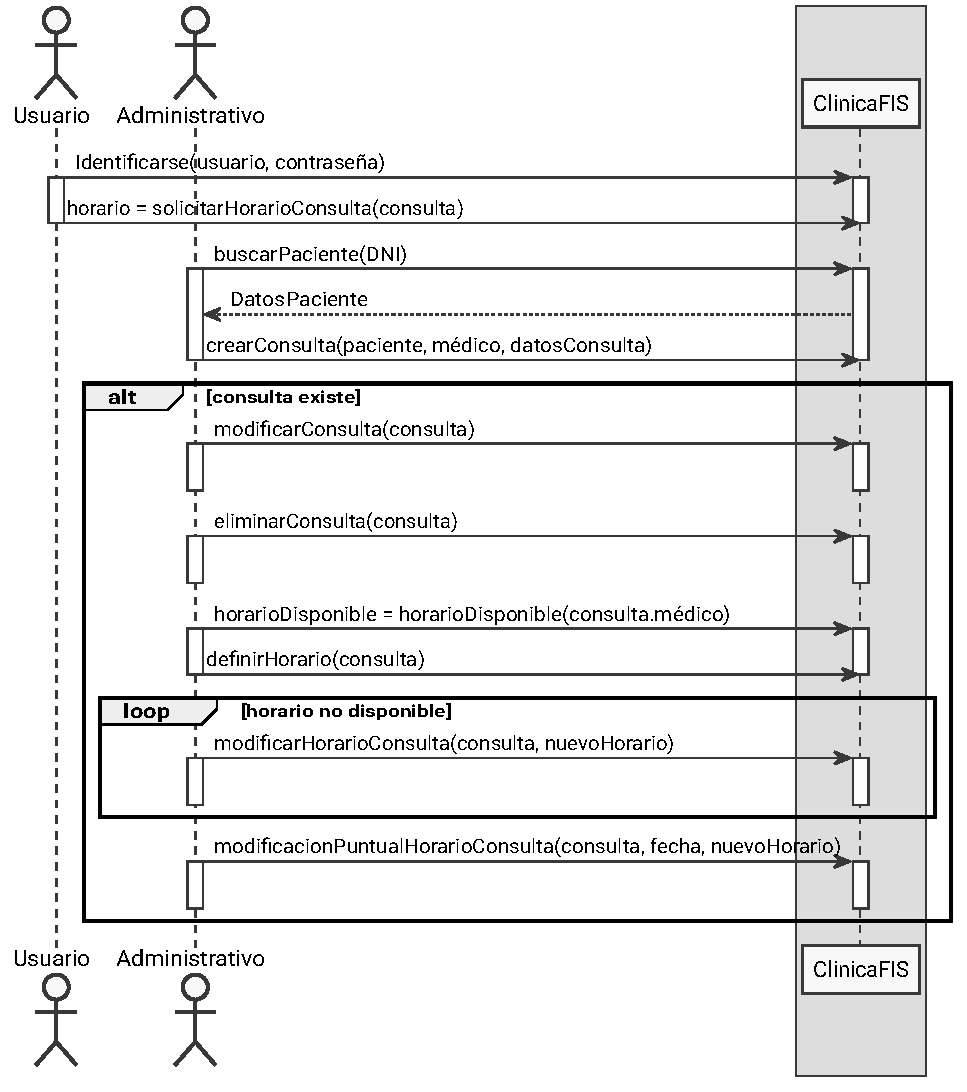
\includegraphics[width=\textwidth,height=\textheight,keepaspectratio]{diagramas/pdf/diagramaGestionConsulta.pdf}
\end{figure}

\begin{figure}[H]
	\caption{Mostrador de consulta}
	\centering
	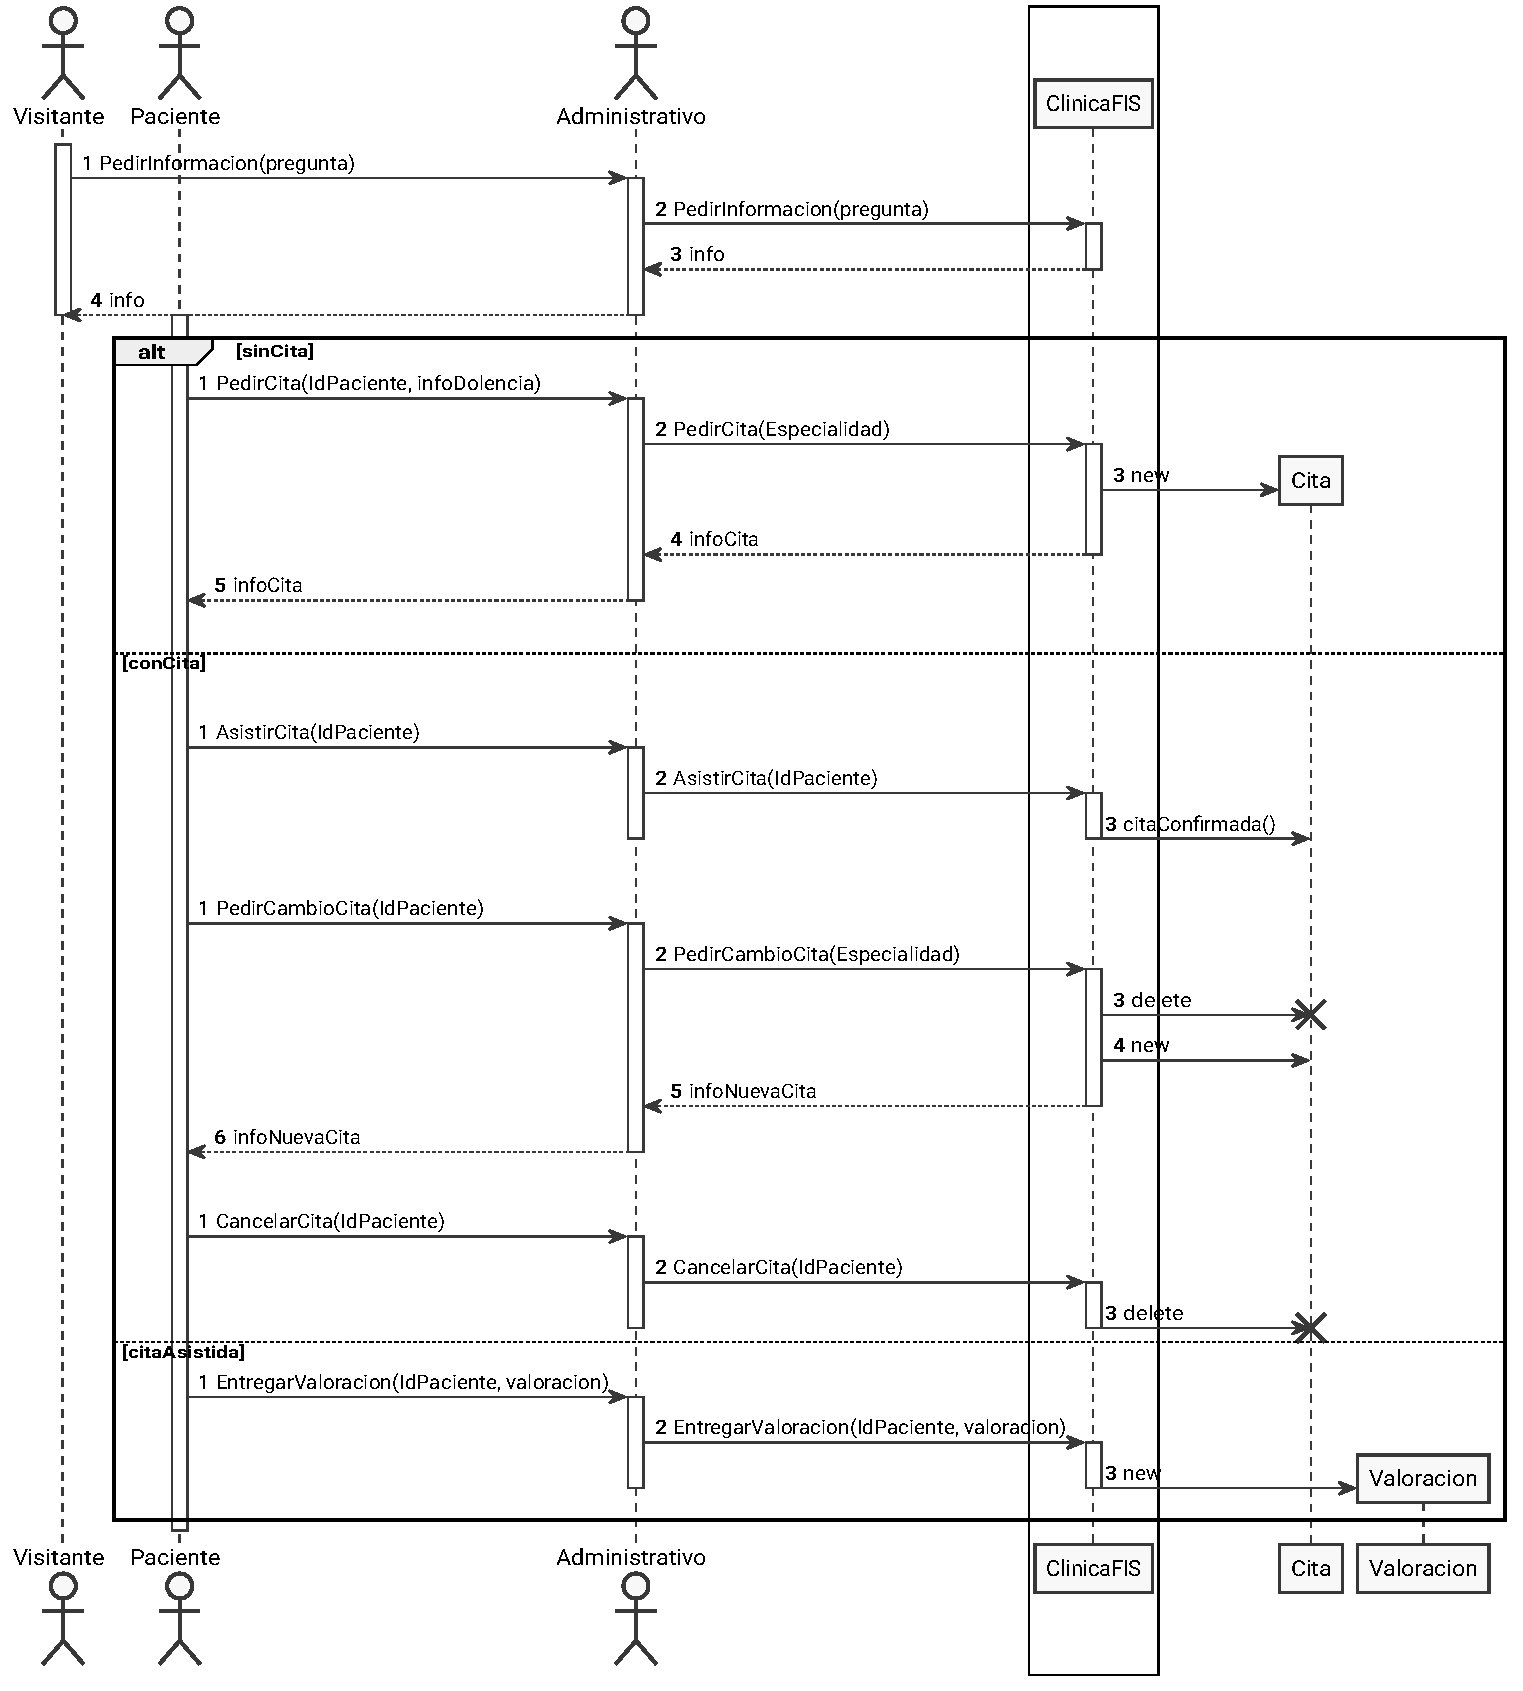
\includegraphics[width=\textwidth,height=\textheight,keepaspectratio]{diagramas/pdf/diagramaMostrador.pdf}
\end{figure}

\begin{figure}[H]
	\caption{Gestión de Pacientes}
	\centering
	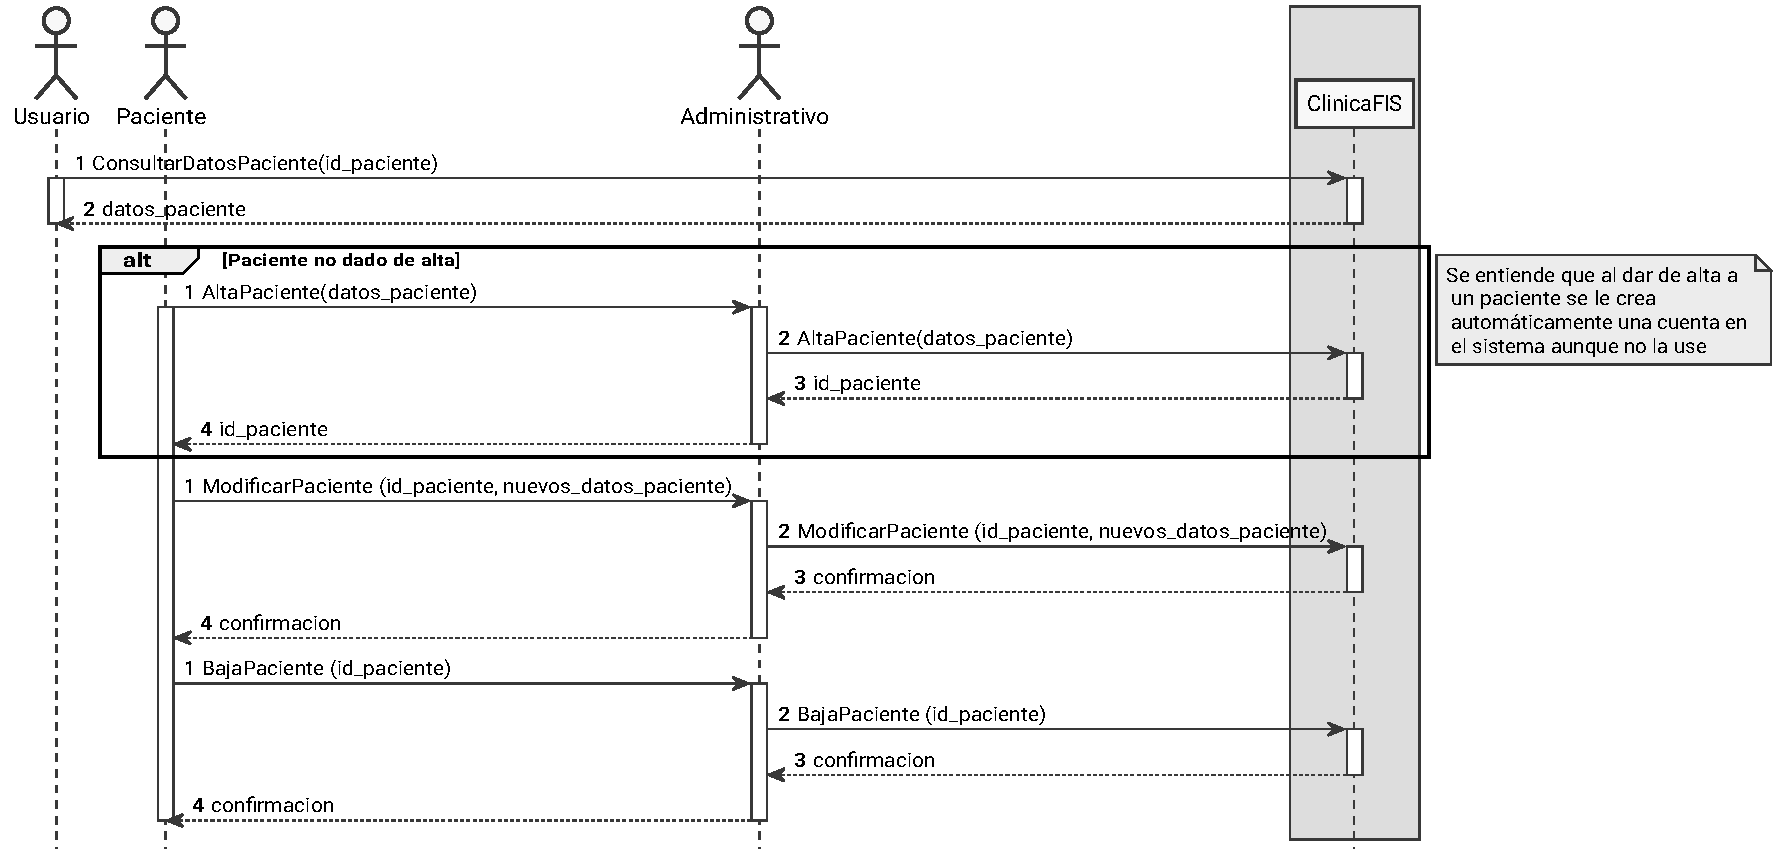
\includegraphics[width=\textwidth,height=\textheight,keepaspectratio]{diagramas/pdf/diagramaPaciente.pdf}
\end{figure}

\begin{figure}[H]
	\caption{Gestión de Personal}
	\centering
	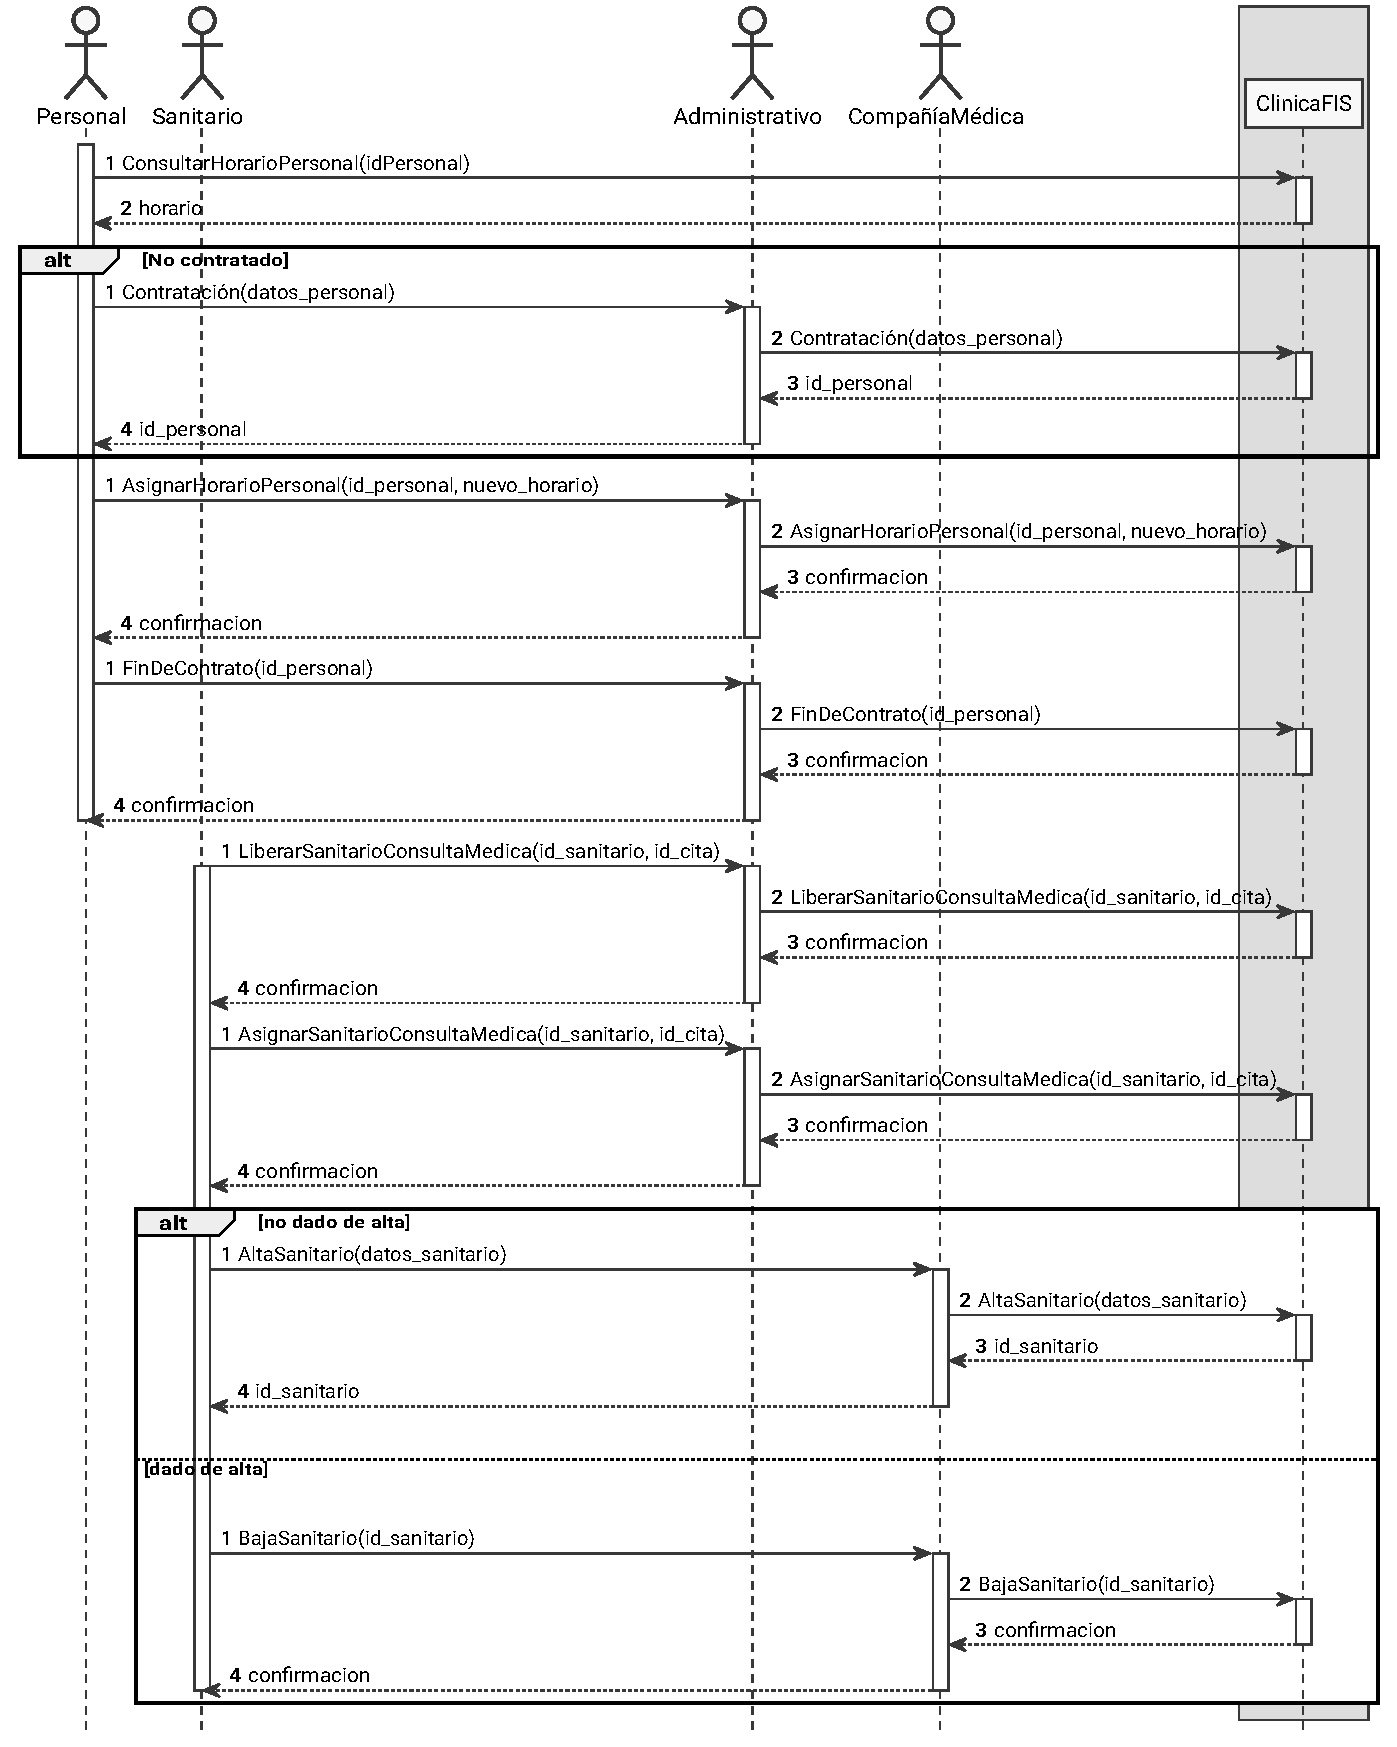
\includegraphics[width=\textwidth,height=\textheight,keepaspectratio]{diagramas/pdf/diagramaPersonal.pdf}
\end{figure}

\begin{figure}[H]
	\caption{Gestión de Recursos}
	\centering
	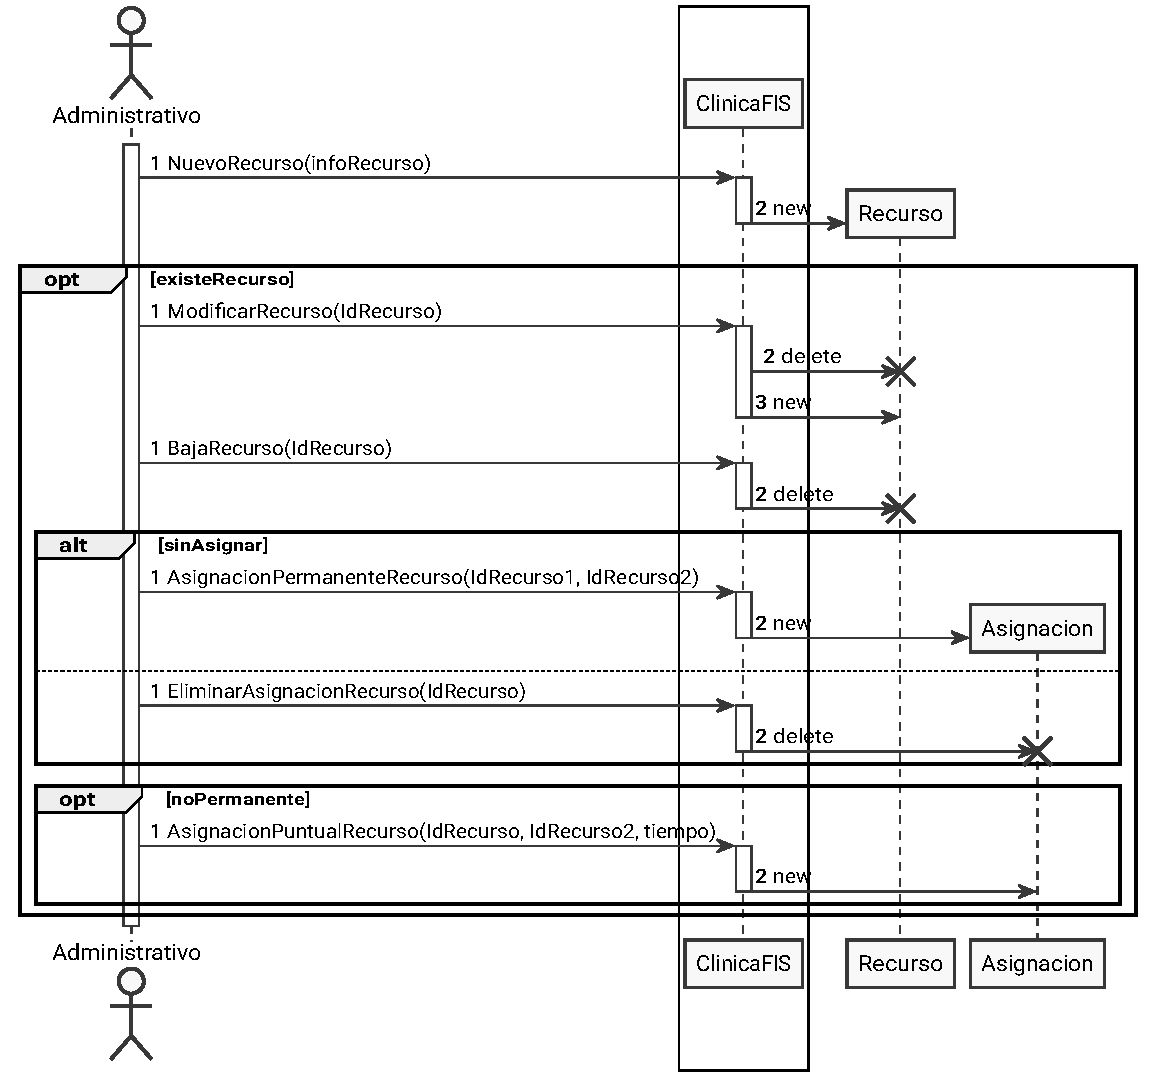
\includegraphics[width=\textwidth,height=\textheight,keepaspectratio]{diagramas/pdf/diagramaRecursos.pdf}
\end{figure}

\begin{figure}[H]
	\caption{Servicio Web}
	\centering
	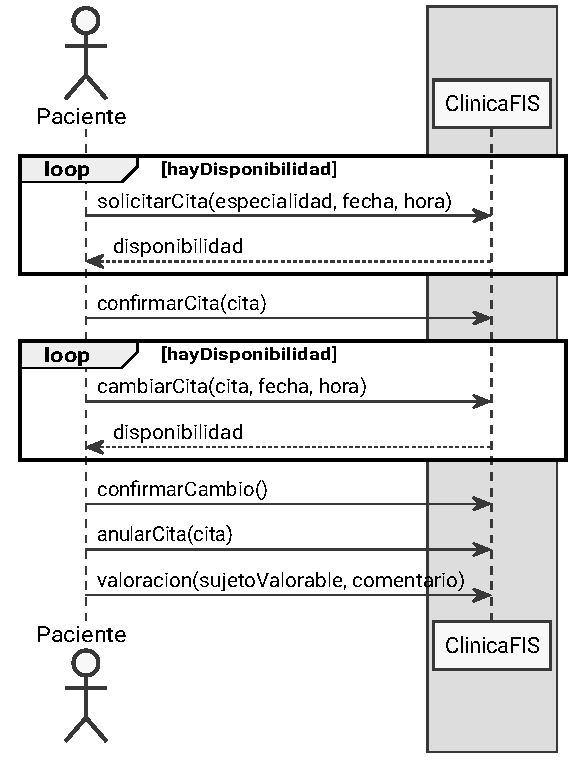
\includegraphics[width=\textwidth,height=\textheight,keepaspectratio]{diagramas/pdf/diagramaServicioWeb.pdf}
\end{figure}

\begin{figure}[H]
	\caption{Unidad de Diagnóstico}
	\centering
	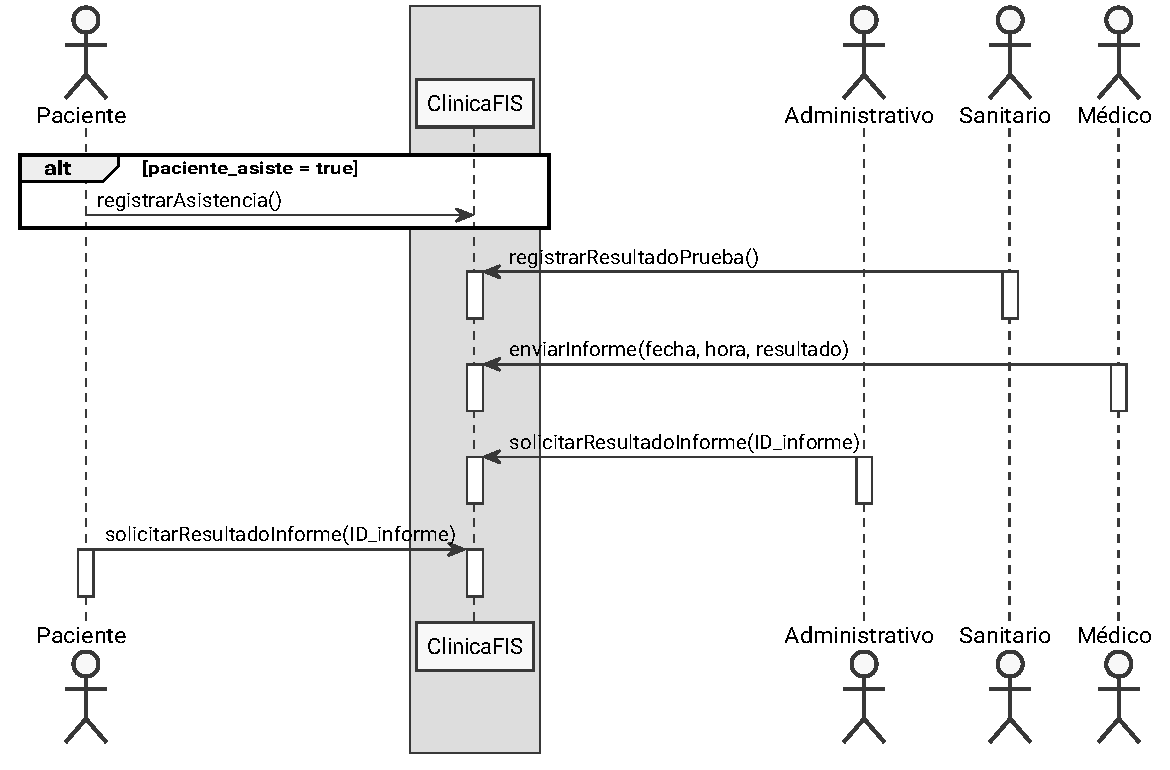
\includegraphics[width=\textwidth,height=\textheight,keepaspectratio]{diagramas/pdf/diagramaUnidadDiagnostico.pdf}
\end{figure}







\end{document}

